\documentclass[a4paper,11pt]{article}
\usepackage{a4wide}%

\usepackage{tabularx}

\usepackage{fullpage}%
\usepackage[T1]{fontenc}%
\usepackage[utf8]{inputenc}%
\usepackage[main=francais,english]{babel}%

\usepackage{graphicx}%
\usepackage{xspace}%
\usepackage{float}
\usepackage{wrapfig}

\usepackage{url} \urlstyle{sf}%
\DeclareUrlCommand\email{\urlstyle{sf}}%

\usepackage{mathpazo}%
\let\bfseriesaux=\bfseries%
\renewcommand{\bfseries}{\sffamily\bfseriesaux}

\newenvironment{keywords}%
{\description\item[Mots-clés.]}%
{\enddescription}

\usepackage[backend=biber, style=authoryear-comp]{biblatex}
\bibliography{Biblio}{}


\newenvironment{remarque}%
{\description\item[Remarque.]\sl}%
{\enddescription}

\font\manual=manfnt
\newcommand{\dbend}{{\manual\char127}}

\newenvironment{attention}%
{\description\item[\dbend]\sl}%
{\enddescription}

\graphicspath{{Figures/}}

\usepackage{listings}%

\usepackage{svg}

\lstset{%
  basicstyle=\sffamily,%
  showstringspaces = false,
  columns=fullflexible,%
  language=c,%
  frame=lb,%
  frameround=fftf,%
}%

\lstMakeShortInline{|}

\parskip=0.2
\baselineskip

\sloppy

%opening
\title{Application des techniques d'appentissage profonds à l'étude de la
  classification de protéines}
\author{Rémy Sun}



\begin{document}

\maketitle

\begin{abstract}
  L'application des techniques d'apprentissage profond à des chaînes peptidiques
  demeure un domaine peu exploré. Nous avons cherché à trouvé des
  caractéristiques importante à l'aide d'auto-encodeurs et avons étudié la
  possibilité d'utiliser des architecture profonde pour la classifictation
  \begin{keywords}
    Deep Learning; Protéines; Séquence
  \end{keywords}
\end{abstract}

\section*{Introduction}

La bonne compréhension des mécanismes régissant le fonctionnement des protéines existantes est un enjeu
important dans de nombreux domaines. %Je peut avoir un exemple?
Cependant il est peu réaliste au vu des moyens actuels de procéder à l'étude
détaillée de tous les mécanismes en jeu pour chaque protéine en raison du coût
élevé des manipulations nécessaires. Néanmoins, nous
disposons d'un grand nombre de séquences peptidiques de protéines, qui influent
directement sur les fonctions d'une protéine.

Les techniques dites d'apprentissage profond ont permis de grand progrès dans de
nombreux domaines qui vont de la reconnaissance d'image à l'étude de langages
naturels (\cite{DBLP:journals/corr/ChoMGBSB14}, \cite{socher2011semi}, \cite{NIPS2014_5346}). Néanmoins, les
protéines demeurent un domaine relativement inexploré par l'apprentissage
profond à l'exception de quelques travaux
(\cite{Spencer:2015:DLN:2817095.2817106}) malgré un certain nombre de travaux
sur l'expression des gènes (\cite{Gupta031906}).

L'applications de techniques dévelloppées en langage naturel ou dans d'autres
branches de la bioinformatique permettent de faire des recoupements sémantiques,
de la classification ou même de la prédiction sur des chaînes de \og mots\fg ou
d'acides aminés. De fait, il semble raisonnable de penser qu'une étude des
protéines avec des techniques similaires devraient permettre de similaires
progrès dans la compréhension des mécanismes gouvernants le fonctionnement des
protéines dont la séquence peptidique est fortement liée au fonctionnement.

Nous nous sommes donc interessés dans ce stage à l'applications de telles techniques
aux familles de protéines. Notre intêret ne portait pas seulement sur la
classification de telles familles ou la reconstitution d'une proteine à partir
d'un séquençage bruité, mais aussi sur l'étude de la possibilité de comprendre
des mécanismes des protéines à partir des représentations intermédiaires acquises par les
algorithmes d'apprentissages profonds entraînés.

\newpage

\section{Apprentissage profond?}

\paragraph{Une technique d'apprentissage machine}

\begin{figure}[!tbp]
\centering  
  \begin{minipage}[b]{0.3\textwidth}
    \includegraphics[width=0.9\textwidth]{Neuron}
    \caption{Exemple de neurone}
  \end{minipage}
\hfill
  \begin{minipage}[b]{0.6\textwidth}
    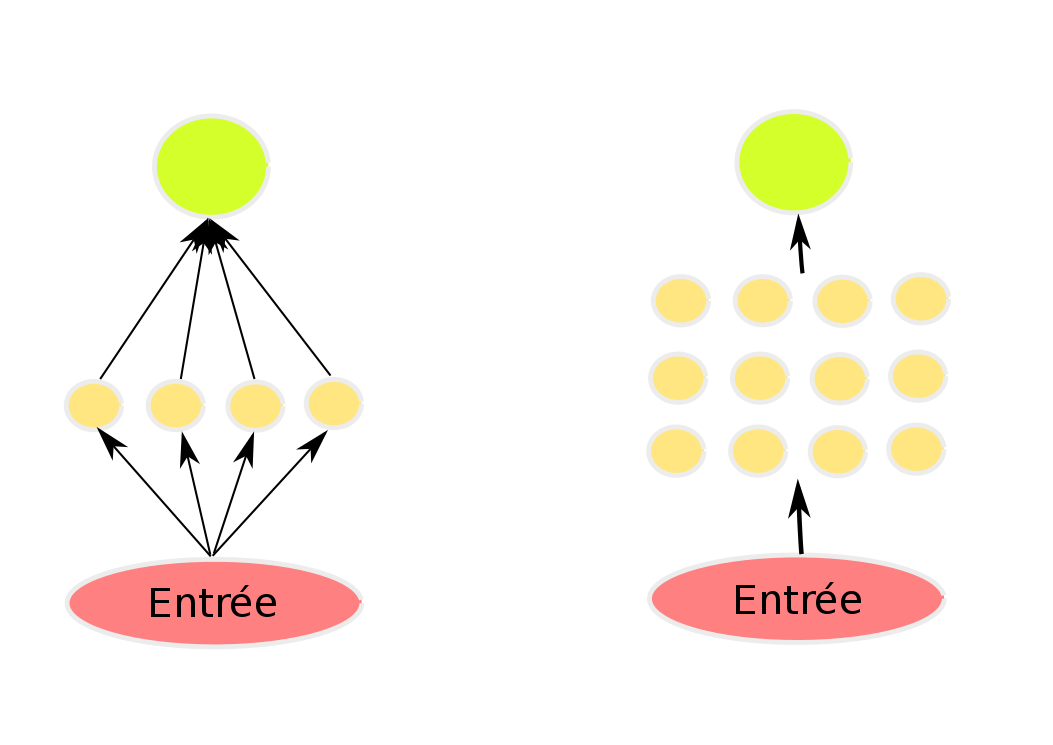
\includegraphics[width=\textwidth]{Deep}
    \caption{Réseau de neurones classique à gauche, Réseau profond à droite}
  \end{minipage}
\end{figure}

Comme toutes les techniques d'apprentissage machine, l'apprentissage profond
vise à entrainer un système pour qu'il résolve des situations sans que tous les
paramètres nécessaires à la résolution du problème n'aient été calculés par
l'implémentateur. Traditionellement, la façon de procéder serait d'utiliser par
exemple un réseau de neurones pour faire un perceptron: il y a un couche entrée,
une couche cachée et une couche sortie. Entre chaque couche une transformation
paramétrée par des variables est effectuée et en sortie on évalue par une
fonction de score le résultat renvoyé. Une optimisation sur les paramètres est
ensuite effectuée, par descente de gradient par exemple.

Ce qui différencie le Deep Learning de ces techniques d'aprentissage dites \og
creuses\fg est d'utiliser plusieurs couches cachées (d'où la notion de
profondeur). Cela augmente remarquablement l'abstraction du problème et permet
de mieux traiter les problèmes dits compositionnels, c'est-à dire qui peuvent se
décomposer en plusieurs composantes. Il est facile en première approximation de
comprendre pourquoi cette façon de procéder est intéressantes: nous comprenons
des choses simples avant de comprendre les choses plus complexes à partir de ce
qui a déjà été appris

\subsection{Entrainement non supervisé}

\paragraph{Autoencodeur}

Une grande problèmatique de l'apprentissage profond est le besoin d'accéder à de
grandes bases de données pour pouvoir entrainer les réseaux. Si cette difficulté
n'est plus d'actualité dans nombreux domaines, elle est indissociable de notre
étude des protéines. Comment faire pour demander à une machine de s'entrainer par elle même sans
qu'on lui dise quelle conclusion tirer à partir de son résultat? Une façon de
faire consiste à lui demander de retrouver son entrée. Ainsi, on ``encode''
l'information dans un premier temps, puis on la décode: c'est l'auto-encodeur.

Traditionellement, c'est à cela (ou aux réseaux basés sur les machines
restreintes de Boltzmann) qu'on fait référence quand on parle d'entraînement
non-supervisé. A strictement parlé, il s'agit plus d'un entraînement
auto-supervisé que non-supervisé, mais aucune réelle méthode d'entrainement
non-supervisée n'existe (il faudrait probablement revoir la structure même de
l'entrainement).

\paragraph{Donc on entraîne un réseau complexe à... retrouver l'identité?}

Ce n'est pas tant le but qui est intéressant ici, mais la façon de l'atteindre.
Evidemment, il y a un réel risque que cette manière de l'atteindre ne soit pas
particuliérement intéressante non plus (on encode l'identité, puis on décode
l'identité). Pour éviter cela on dispose de plusieurs moyens:

\begin{itemize}
\item Forcer l'encodeur à encoder l'entrée en une représentation intermédiaire
  de dimension inférieure. Ainsi, on s'assure de ne pas pouvoir juste propager
  l'identité. Mieux encore, la représentation intermédiaire, ``condensée'' peut
  permettre de découvrir des ``points robustes'' de ce qu'on est en train
  d'apprendre. Ce qui caractérise une famille de protéines par exemple...
  Néanmoins, le grand défaut de cette approche est que la perte d'information
  est ici inévitable.
\item Corrompre l'information donnée en entrée (comme proposé par \cite{Vincent:2008:ECR:1390156.1390294})pour forcer l'encodeur à
  ``deviner'' ce qu'il manque, ce qui permettrait par exemple de mettre en
  lumière des corrélations non évidentes à l'oeil nu.
\item Poser des contraintes sur la représentation intermédiaire acquise
\item Aléatoirement désactiver certains neurones, ce qui force le système à
  introduire de la redondance (et donc à choisir ce qui est réellement
  important). C'est une technique aussi employée dans d'autres réseaux neuronaux
  pour éviter de spécialiser le réseau sur l'ensemble d'entraînement et non sur
  le domaine où on veut l'appliquer. Il est raisonnable qu'un auto-encodeur
  entrainé sur des familles de protéines gére mal les chaînes purement
  aléatoires, mais il serait problèmatique que cet auto-encodeur n'arrive pas à
  traiter des protéines proches des exemples d'entraînement mais n'en faisant
  pas partie. En effet, si on veut catégoriser les pompiers, et que par hasard
  tous ceux de l'exemple d'entraînement sont bruns, il y a un risque d'associer
  pompier et brun.
\end{itemize}

Une partie de notre travail s'est focalisée sur l'étude de ces représentations
intermédiaires et sur ce qu'elles nous apprennent sur les familles de protéines
ayant servi à l'entraînement de l'auto-encodeur.

\subsection{Réseaux convolutifs}

\paragraph{Il y a un motif caractéristique (feature) dans les images d'oiseaux}

C'est probablement intéressant pour classifier des images d'animaux, mais de là
à le repérer sur un pixel... Ce qu'on peut faire par contre, est \og
scanner\fg des carrés $3\times 3$. En pratique, c'est créer une couche cachée
dont chaque neurone applique une même transformation sur les 9 neurones d'un
carré $3\times 3$. Il s'agit donc de faire une convolution sur l'image d'une
fonction de transformation!

Nous venons de décrire une couche générant une image réduite dont chaque
neurone/pixel donne la valeur de l'application d'une fonction à un carré
$3\times 3$. Nous appellerons une telle représentation \texttt{feature map}:
elle donne la représentation d'une \og feature\fg sur l'image.

\paragraph{Pourquoi s'arrêter à une \texttt{feature map}?}

Typiquement on crée plusieurs \texttt{feature maps} en parrallèle dans un réseau
convolutionnel. Rappellons déjà que nous n'avons pas beaucoup de contrôle sur la
caractèristique que le réseau va retrouver puisqu'il va apprendre la
caractéristique qui donne le meilleur résultat par lui-même. Multiplier les
\texttt{feature maps} permet de distinguer plus de points caractéristiques qui
seront ensuite traités par une couche supérieure.

Si on veut rajouter une couche convolutionnelle au dessus, elle opérera non
seulement une opération sur un carré de chaque \texttt{feature map}, mais elle
effectura une opérations sur les résultats de cette opération sur chaque feature
map.

\paragraph{Réduire la charge de calcul}

Pour augmenter un peu la robustesse du système à une translation par exemple, on
effectue un \texttt{pooling} qui consiste à regrouper ensemble des blocs de
neurones. Non seulement cela permet de réduire la taille de la représentation
considérée, cela fait qu'une simple translation a moins de chance de changer
quoi que ce soit à l'image obtenue après transformation.

\begin{figure}
  \centering
  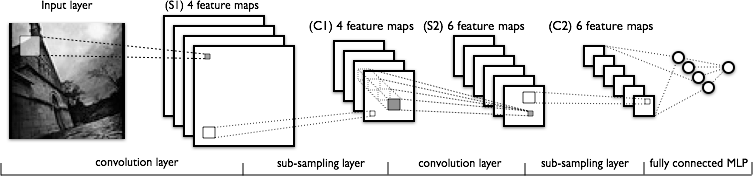
\includegraphics[scale=0.8]{mylenet}
  \caption{Réseau convolutionnel LeNet5}
\end{figure}

Une architecture typique se constitue donc d'un enchaînement de couches de
convolution et de pooling, avec une ou plusieurs couches \og classiques\fg
permettant de tirer une conclusion sur les information récupérées. Une telle
architecture est proposée dans \cite{lecun1998gradient} sous la forme du réseau LeNet5

\subsection{Réseaux récurrents}

\paragraph{Il est utile de se rappeler des mots précédents à la lecture d'une phrase}

L'idée est que l'entrée est traitée comme une suite d'entrées:
typiquement c'est le cas d'une phrase par exemple. Chaque mot est traité par la
couche récurrente qui va calculer deux choses à partir de cette entrée: une
sortie \og publique\fg et une sortie caché qui détermine un paramètre de la
couche (une sorte d'état interne caché). Le second élément de la suite est
ensuite traité par ce même neurone dont l'état caché a évolué suite au
traitement du premier élément de la suite.

Si on \og déplie\fg l'exécution du problème, on réalise que la séquence passe en
fait par un nombre de couches cachées égal au nombre d'éléments dans la suite!
Ainsi, nous avons établit un réseau qui est capable de traiter un élément d'une
suite en se rappelant en quelque sortes de ce qui s'est passé avant. La seule
question qui reste à traiter est le fonctionnement exact de la couche cachée.

Il est possible de faire fonctionner cette couche cachée comme un réseau neuronal
complétement relié classique avec une sortie et entrée supplémentaire
représentant l'état caché, mais cela pose d'est problème d'évanouissement du
gradient lors de la rétropropagation.

\begin{figure}[!tbp]
  \centering
  \begin{minipage}[b]{0.45\textwidth}
    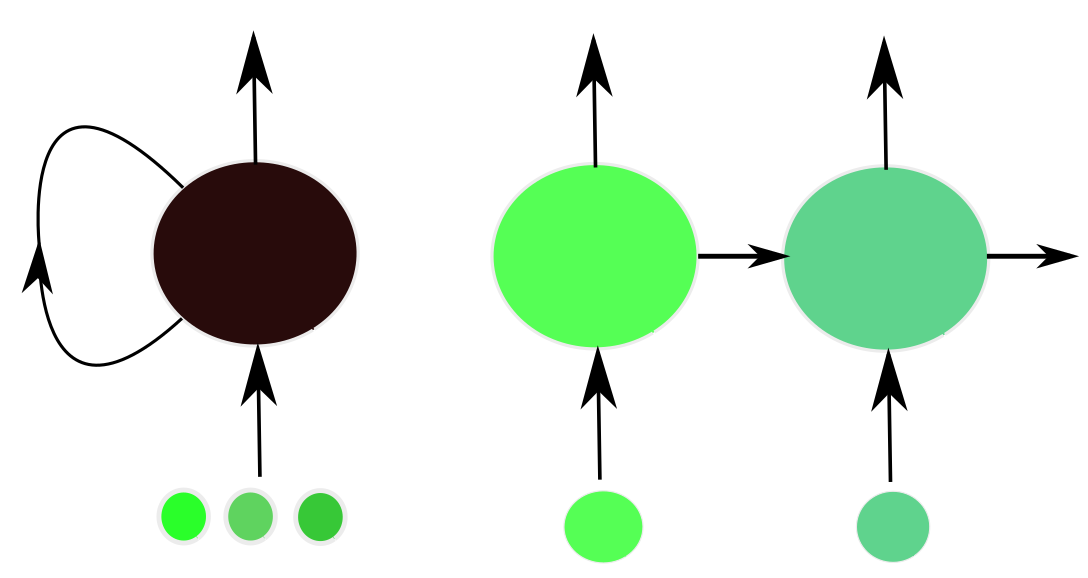
\includegraphics[width=\textwidth]{Recurrent}
    \caption{Réseau récurrent à gauche, forme dépliée temporellement à droite}
  \end{minipage}
  \hfill
  \begin{minipage}[b]{0.5\textwidth}
    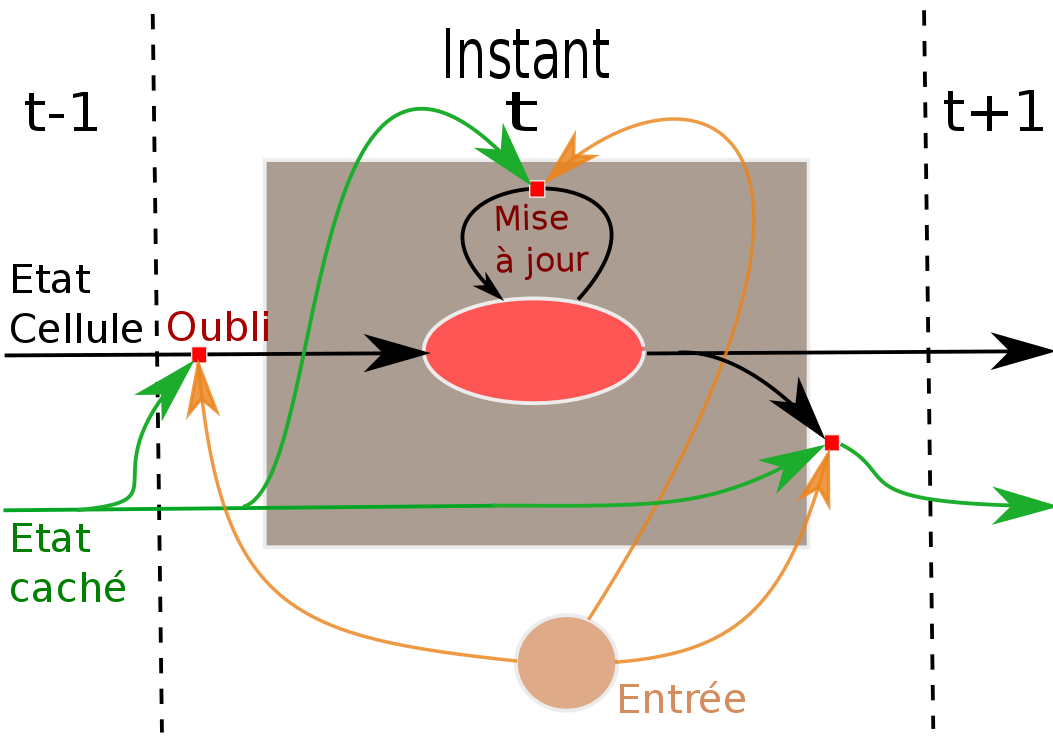
\includegraphics[width=\textwidth]{LSTM}
    \caption{Exemple d'unité LSTM}
  \end{minipage}

\end{figure}

\paragraph{Long Short-Term Memory (LSTM)}

Une architecture de couche dont le comportement naturel est de se rappeler de ce
qui s'est passé avant est exposée dans . L'idée est qu'on a un état de
cellule, un état caché et une entrée. A chaque passage dans la couche, on calcule
quel degré d'information il faut retenir de l'état de la cellule en fonction de
l'état caché et de l'entrée. Ensuite on calcule s'il faut ajouter de
l'information à l'état de la cellule. Enfin, on fait le calcul de la sortie et
de l'état caché à partir des trois données précedentes.

\paragraph{Pourquoi utiliser un réseau récurrent?}

Les réseaux récurrents se sont avérés très utiles à l'études du langage naturel
puisqu'il permettent de détecter des corrélations dans une phrase qu'un réseau
convolutionnel ne détecterait pas forcément (la fenêtre de détection d'une
couche convolutionnelle est après tout de taille finie).  La sortie récupérée
peut être de deux types différents: on peut récupérer la suite des sorties du
réseau récurrent, ou on peut choisir de récupérer la dernière sortie de la
couche récurrente qui servirait alors de \og résumé\fg de ce qui s'est passé à
la lecture de la suite.

\paragraph{Un auto-encodeur récurrent?}

Une architecture d'auto-encodeur profonde que nous avons particulièrement étudié
(et qui fournit de bons résultats pour la détection de structures comme la copie
dans une chaîne) est celle proposée dans \cite{DBLP:journals/corr/ChoMGBSB14}.
L'idée est d'utiliser un premier auto-encodeur pour servir d'encodeur: on ne
récupére que sa sortie sur le dernier terme de la suite d'entrée. Cette sortie
est de dimension finie et nous servira de résumé (qui compresse éventuellement
l'information). Il suffit ensuite de passer ce résumé dans un autre
auto-encodeur récurrent en récupérant cette fois chaque sortie (qu'on encode
ensuite en une lettre avec un réseau dense et un \texttt{softmax}). Dans
l'article original, la sortie du décodeur au temps $t$ lui est aussi donné en
entrée au temps $t+1$, mais ce n'est pas le cas dans notre étude.

\subsection{Initialisation et optimisation des réseaux d'apprentissage profond}

\paragraph{Entraînement non-supervisé?}

Il a été montré dans de nombreux travaux qu'il est possible d'entrainer des
auto-encodeurs les uns à la suite et d'aboutir à des situations permettant
d'éviter de trop mauvais minima locaux. C'est d'ailleurs ce qui a motivé le
second souffle du deep learning vers la fin des années 2000

Néanmoins, des travaux plus récents ont montrés qu'il suffit d'utiliser des
initialisation aléatoires bien choisies pour largement passer outre les problème
de minima locaux quand l'ensemble d'apprentissage est de taille élevée: nous n'avons jamais besoin que d'une instance d'entraînement
évitant les minima locaux. Nous avons utilisé dans ce stage l'initialisation
proposée dans . Cependant, nous avons aussi dû travailler avec des jeux de
données de taille faible, ce qui a nécéssité le passage par de l'apprentissage
non-supervisé.

\paragraph{Rétropropagation}

Nous disposons d'une fonction de score en fin de réseau. Notre but est de
minimiser cette fonction en modifiant les paramètres internes du réseau (qui
déterminent les transformations effectuées sur l'entrée.). Pour ce faire, on
utilise typiquement le gradient de la fonction de coût. Cela peut se faire au
travers de quelquechose d'aussi simple que la descente de gradient stochastique, mais cette
dernière a de nombreux défauts. Dans cette article nous utiliserons les
optimisations dites \texttt{adagrad} (très efficace dans les réseaux
convolutifs) et \texttt{RMSProp} (très efficace dans les réseaux récurrents).

\paragraph{De la non linéarité}

En un sens, les réseaux neuronaux cherchent à observer les données \og sous un
certain angle\fg qui permet de trouver des corrélations: cela permet de faire de
la classification, de la reconstruction, voire de la prédiction. Néanmoins si on
se borne à effectuer des opérations linéaires (sommes pondérées
d'entrés, trnasformations affines) il est tout a fait possible de passer à coté
d'un regroupement intéressant des points (les fonction linéaire préservent
notemment l'alignement ce qui peut se révéler être un grand problème). De fait,
il y a toujours \og à la fin\fg d'une couche une fonction dite \og
d'activation\fg qui opére une transformation non-linéaire sur la sortie.
Traditionnellement, on applique une sigmoïde ou une tangente hyperbolique, mais
Hinton a montré qu'il est plus judicieux d'utiliser une fonction de seuillage \texttt{ReLU}.

\section{Travail réalisé}

\subsection{Matériel}

Nous avons effectué l'ensemble de nos travaux à l'aide librairies python.

Pour ce qui est de l'aspect apprentissage profond, nous avons principalement
utilisé \texttt{keras} (\cite{chollet2015keras}) qui est une libraire haut niveau
permettant de manipuler facilement des couches d'apprentissage. Ce choix vient
d'une part de la nature des problèmes étudiés qui nous mènent à tenter
l'utilisation de plusieurs architectures (ce qui invalide des librairies comme
Caffee pour C++ spécialisé en réseaux convolutifs) et de l'autre de la grande
souplesse offerte par Keras. En effet, \texttt{keras} peut utiliser deux
librairies bas niveau python (il est possible de choisir entre les deux): le
grand classique \texttt{Theano} (\cite{2016arXiv160502688full}) et le plus récent
\texttt{Tensor Flow} (\cite{tensorflow2015-whitepaper}) de Google.

Pour ce qui est de la manipulation de séquence peptidiques à proprement parlé,
nous avons utilisé des données de la base de donnée \texttt{SCOPe}
(\cite{fox2014scope}) et la librairie python Biopython (\cite{Cock01062009})

\subsection{Représentation des chaînes peptidiques}

Ce qui a été fait à de maintes reprises par le passé est la représentation des
protéines non pas comme chaines d'acides, mais comme un vecteur dépendant de
différents paramètres. Ces paramètres vont de notions simplistes comme le nombre
d'occurence de chaque acide aminé dans la chaîne à des considérations beaucoup
plus complexes comme l'étude des fonctions de la protéine.

Notre travail s'est principalement basé sur l'étude de proteines en tant que
chaîne d'acides aminés représentés par des lettres. En quelque sorte, nous traitons donc des suites de \og
mots\fg. De fait, il est nécessaire de déterminer une façon de représenter ces
différents mots. Il est facile de voir pourquoi la première idée de simplement
indexer les acides par des entiers est problématique: pourquoi la lettre \og
A\fg serait elle plus proche du \og B\fg que du \og Z\fg? Pour résoudre ce
problème, nous nous sommes intéréssés à ce qui a été en traitement de langages
naturels.

Une représentation répandue, bien qu'assez simpliste consiste à créer un espace
contenant autant de dimensions qu'il y a d'acides aminés et représenter chaque
acide aminé par un vecteur d'une base orthogonale de cet espace. Plus
simplement, cela veut dire qu'on représente chaque acide par un vecteur ne
contenant que des 0 et un 1. Cette représentation permet d'avoir des résultats,
mais elle présente en langage naturel l'inconvénient d'engendrer une
représentation dans l'espace très lacunaire, ce qui crée des espaces inutilement
grands. Ce problème est secondaire dans notre cas puisqu'il n'y a qu'une
vingtaine d'acides à considérer.

Néanmoins, il est intéressant de remarquer que des outils ont été inventés en
langages naturels pour passer outre ce problème. L'idée est d'apprendre un
représentation de dimension inférieure distribuée prenant en compte les mots
apparaissant généralement avec celui considéré. Cela se fait avec des techniques
d'apprentissages qui cherchent à maximiser le score de phrases valides et
minimiser celui de phrases non valides. Ces techniques ne sont pas applicables à
notre problème à cause de la façon dont les séquences peptidiques fonctionnent,
mais nous avons voulu retenir l'idée qu'on peut placer les acides dans un espace
de dimension faible en tenant compte de leur spécificités. En regardant 4
propriétés physico-chimiques, nous avons donc créé une telle représentation.
L'aspect important d'une telle représentation est qu'elle permet de justifier du
fait que deux acides sont proches du point de vue de leur représentation, ou du
fait que trois acides sont equidistants. En effet, la représentation précédente
posait le problème inverse de l'indexage: pourquoi tous les acides sont-ils équidistants?

\subsection{Choix des architectures d'apprentissage profond}

Dans le cadre du traitement de séquences peptidiques, il semble tout indiqué
d'utiliser des réseaux récurrents puisqu'une structure temporelle semble
apparaître dans l'enchaînement des acides aminés. Néanmoins, le grand défaut de
réseaux récurrent est que, contrairement aux réseaux profonds dits \og
classiques\fg, ils repérent des dépendances temporelles et non hiérarchiques.
Pour pallier à ce problème, il semble nécessaire d'empiler les réseaux
récurents, ce qui a vite des conséquences significatives en termes de temps de
calculs dès qu'on traite des séquences un peu longues.

Une autre architecture intéressante est celle des réseaux convolutionnels
exposés plus haut. Dans la façon de procéder décrite plus haut, un acide aminé
est traité comme un \og mot\fg. Cela ne correspond pas nécéssairement à une
quelconque réalité, à moins qu'on pense qu'une lettre est un mot. Il n'existe
cependant pas de moyen d'extraire à priori un \og mot\fg (un groupe d'acides)
d'une chaîne peptidique: il n'y a pas d'acide \og séparateur\fg. Cependant, les
réseaux convolutionnels offrent un moyen alternatif de repérer ces mots: si une
\texttt{feature map} est appliquée sur 7 acides, alors cette \texttt{feature
  map} sera capable de repérer (après entraînement) un mot (caractéristique) de
longueur inférieure ou égale à 7.

\subsection{Etude préliminaire sur séquences artificielles}

Nous avons généré aléatoirement plusieurs jeux de données pour comparer les
capacités de diverses architectures d'auto-encodeurs et classificateurs. Nous
avons testé deux types de jeux de données: un jeu de données où la première
moitié de la chaine est fixée et où la seconde moitié est telle que chaque
lettre est tirée avec probabilité uniforme; et un jeu de données où la premiére
moitié est tirée avec probabilité uniforme sur chaque lettre et où la seconde
moitié est égale à chaque moitié.

\subsubsection{Auto-encodeurs}

Nous envisageons principalement deux architectures d'encodeurs: un réseau
convolutionnel (à couche multiples) et un réseau récurrent LSTM (à une ou plusieurs
couches) dont nous récupérons la dernière sortie. Le décodeur est dans tous les
cas un réseau récurrent LSTM.

Les deux architectures n'ont aucun problème à repérer la caractéritique des données dont le
début est fixé, ce qu'elle reconstitue très bien. Par contre, il semble que l'architecture dont l'encodeur est un
réseau convolutionnel ne parvient pas à décoder correctement les caractères
aléatoires. De plus, il ne semble même pas repérer la relation de \og copie\fg
présente dans le second jeu de données. Au contraire, il semble que l'encodeur
récurrent, même à une seule couche apprend très vite à créer des mots dont les
deux moitiées sont très similaires, même si elles n'ont pas grand chose à voir
avec l'entrée réelle. Sous condition de disposer d'un temps d'entraînement assez
long, l'encodeur récurrent permet aussi de reconstituer correctement les
caractéres tirés aléatoirement.

\subsubsection{Classificateurs}


\subsection{Clustering de protéines}

Les auto-encodeurs générent un représentation intermédiaire dans un premier
temps. Nous avons voulu étudier cette représentation intermédiaire pour en
apprendre plus sur les choses auquelles l'auto-encodeur fait attention quand il
encode la protéine et qui lui permettent de reconstruire par la suite la
protéine. \cite{jian2013predicting} a déjà été effectuée sur la capacité de réseaux d'auto-encodeurs
empilés à classifier la structure secondaire de protéines, mais cette étude ne
s'est malheureusement pas attardé sur le problème de la représentation intermédiaire.

En première approximation, on pourrait penser retrouver un hyperplan ou une
nappe aparentable à une feature connue. Néanmoins une telle étude est difficile
à exploiter. Nous nous sommes penchés sur la piste du clustering
de protéines en fonction de leur représentation intermédiaire. En effet, si on
regroupe ensemble des protéines \og proches\fg du point de vue de leur
représentation intermédiaire, il est peut-être possible de remarquer
des points remarquables dans la structure de protéines qui pourront être
ré-utilisés de manière indépendante de l'apprentissage profond plus tard.

Un simple algorithme de K-means permet de faire le découpage en parties de
l'ensemble d'apprentissage.

\section{Vérification}

\section{Contribution}

\section*{Conclusion}

\printbibliography

\end{document}
